%% Requires compilation with XeLaTeX or LuaLaTeX
\documentclass[10pt,xcolor={table,dvipsnames},t]{beamer}
\usetheme{}

\title[Your Short Title]{Indoor Tracking App}
\subtitle{GPS less tracking system}
\author{Lionel Cominelli}
\institute{Universit� de la R�union / Master 1 informatique}
\date{10/12/2021}

\begin{document}

\begin{frame}
  \titlepage
\end{frame}

% Uncomment these lines for an automatically generated outline.
%\begin{frame}{Outline}
%  \tableofcontents
%\end{frame}

\section{Introduction}

\begin{frame}{Plan}

\begin{itemize}
  \item {\Large Problematic}
  \item {\Large The App solution}
  \item {\Large Zoom on inertial principle}
  \item {\Large The implementation}
  \item {\Large Perspectives }
\end{itemize}

\end{frame}



\begin{frame}{Problematic}

{\large Since the 2001, US government has open the Global Positioning System (GPS) military tracking system to the world. \\ 
- \\
People take possession of the technology and intensively use it.\\ 
- \\


Today, we cannot imagine living without GPS ! \\ 
- \\ 


GPS works with satellites and outcomes your position by distance triangulation between you and the satellites. \\ 
- \\

But, what's happen inside a building ???? \\ 
- \\

GPS does not work.... to keep tracking indoor we must find another way.  }

\end{frame}


\begin{frame}{The App Solution}

\includegraphics[width=.5\textwidth,height=.5\textheight]{indoortracking.jpg}

\begin{itemize}
  \item {Init button : reset the displayed track, localize the position in the center of the screen}
  \item {GSP button : reset the displayed track and localize the position into a background map}
  \item {Button QR ; reset the displayed track and localize the position into a building background map}
  \item {The track : the path performed by the user}
\end{itemize}


\end{frame}


\begin{frame}{Zoom on inertial principle}
\begin{itemize}
  \item {\Large How the position is determined without GPS ?}
\end{itemize}
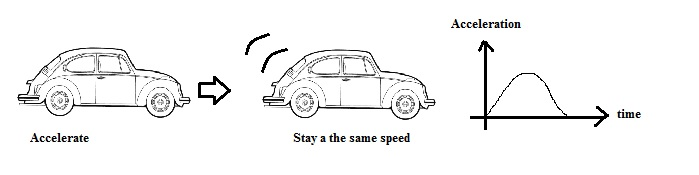
\includegraphics[width=1.0\textwidth,height=0.45\textheight]{a1.jpg}


\end{frame}


\begin{frame}{Zoom on inertial principle}
\begin{itemize}
  \item {\Large How the position is determined without GPS ?}
\end{itemize}

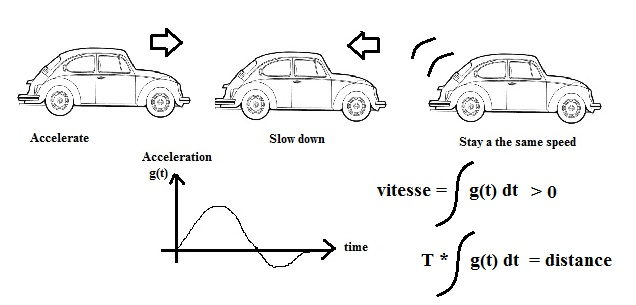
\includegraphics[width=1.0\textwidth,height=0.8\textheight]{a2.jpg}
\end{frame}

\begin{frame}{Zoom on inertial principle}
\begin{itemize}
  \item {\Large How the position is determined without GPS ?}
\end{itemize}
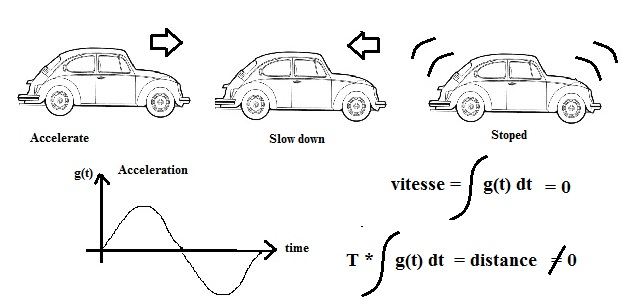
\includegraphics[width=1.0\textwidth,height=0.8\textheight]{a3.jpg}
\end{frame}

\begin{frame}{Zoom on inertial principle}
\begin{itemize}
  \item {\Large How the position is determined without GPS ?}
\end{itemize}
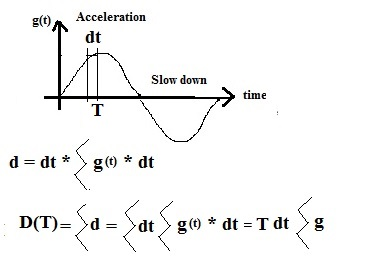
\includegraphics[width=1.0\textwidth,height=0.8\textheight]{a4.jpg}
\end{frame}

\begin{frame}{The implementation}
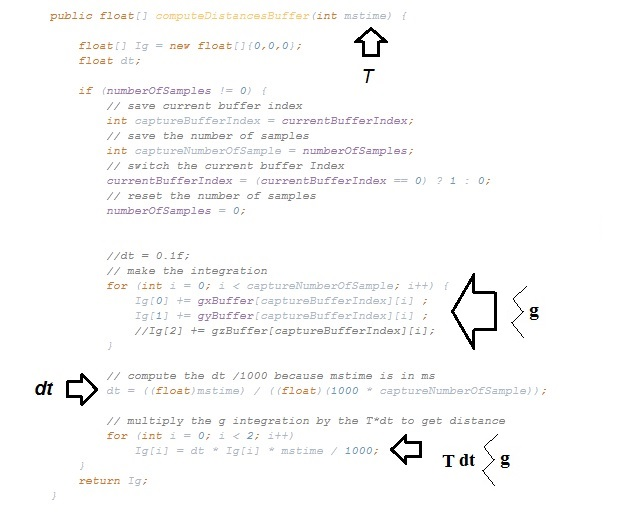
\includegraphics[width=1.0\textwidth,height=0.8\textheight]{code1.jpg}
\end{frame}

\begin{frame}{The implementation}
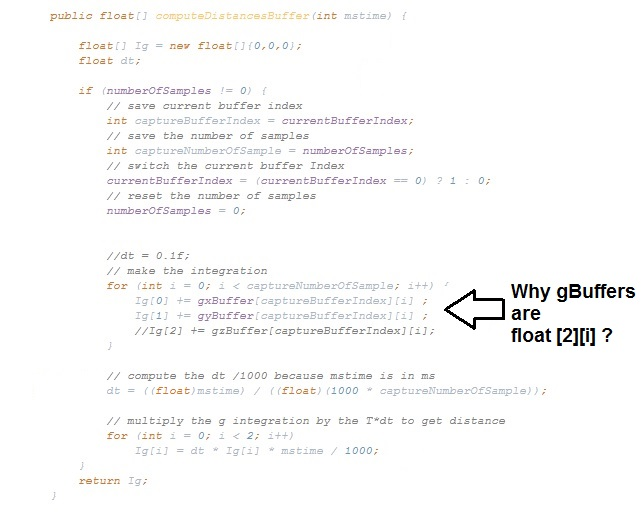
\includegraphics[width=1.0\textwidth,height=0.8\textheight]{code2.jpg}
\end{frame}

\begin{frame}{The implementation}
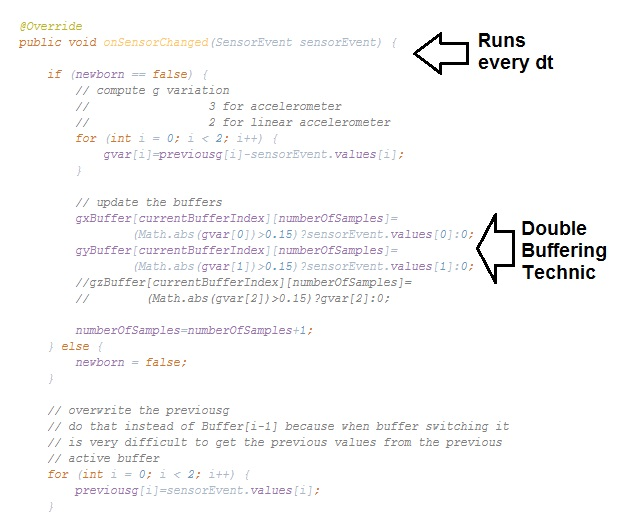
\includegraphics[width=1.0\textwidth,height=0.8\textheight]{code3.jpg}
\end{frame}

\begin{frame}{Perspectives}
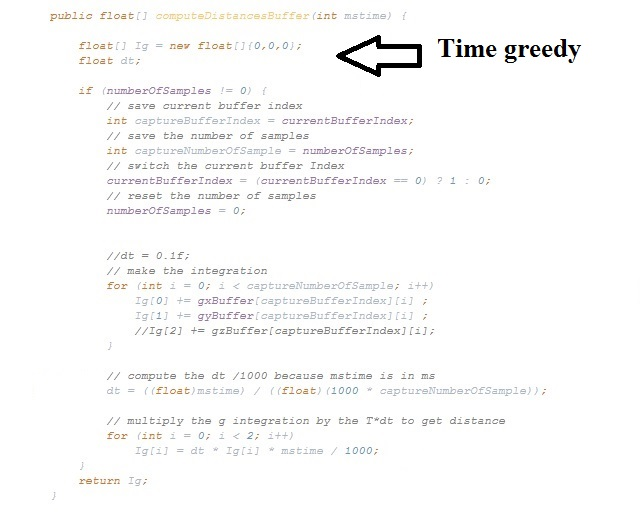
\includegraphics[width=1.0\textwidth,height=0.8\textheight]{code4.jpg}
\end{frame}


\begin{frame}{Perspectives}
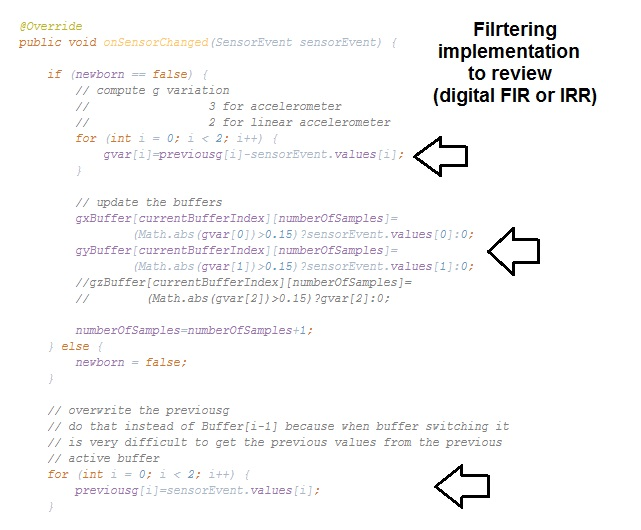
\includegraphics[width=1.0\textwidth,height=0.8\textheight]{code5.jpg}
\end{frame}

\begin{frame}{Conclusion}
\begin{itemize}
  \item {Accelerometer very sensitive}
  \item {Sensor driver implementation must be meticulous}
  \item {Embedded software is a real trade }
  \item {GUI Design too !}
\end{itemize}


\end{frame}

\begin{frame}{Thank you}



\end{frame}



\end{document}
